\documentclass[../main.tex]{subfiles}
\graphicspath{{\subfix{../image/}}}
\begin{document}
\begin{frame}{Tâm lý học Kĩ thuật - Phương pháp nghiên cứu}
\subsection{Phương pháp nghiên cứu}
Tâm lý học kỹ thuật tập trung vào việc hiểu sâu hơn về tương tác giữa con người và công nghệ. Cụ thể hơn, các phương pháp nghiên cứu chính của ngành bao gồm:
\begin{itemize}
    \item Hành vi của con người khi sử dụng công nghệ.
    \item Các yếu tố tâm lý ảnh hưởng đến việc sử dụng công nghệ.
    \item Thiết kế các hệ thống công nghệ.
    \item Ảnh hưởng của công nghệ đến tâm lý con người.

\end{itemize}

\end{frame}

\begin{frame}{Tâm lý học Kĩ thuật - Một số trung tâm nghiên cứu hàng đầu}
    \begin{minipage}{0.5\textwidth}
        \begin{figure}
            \centering
            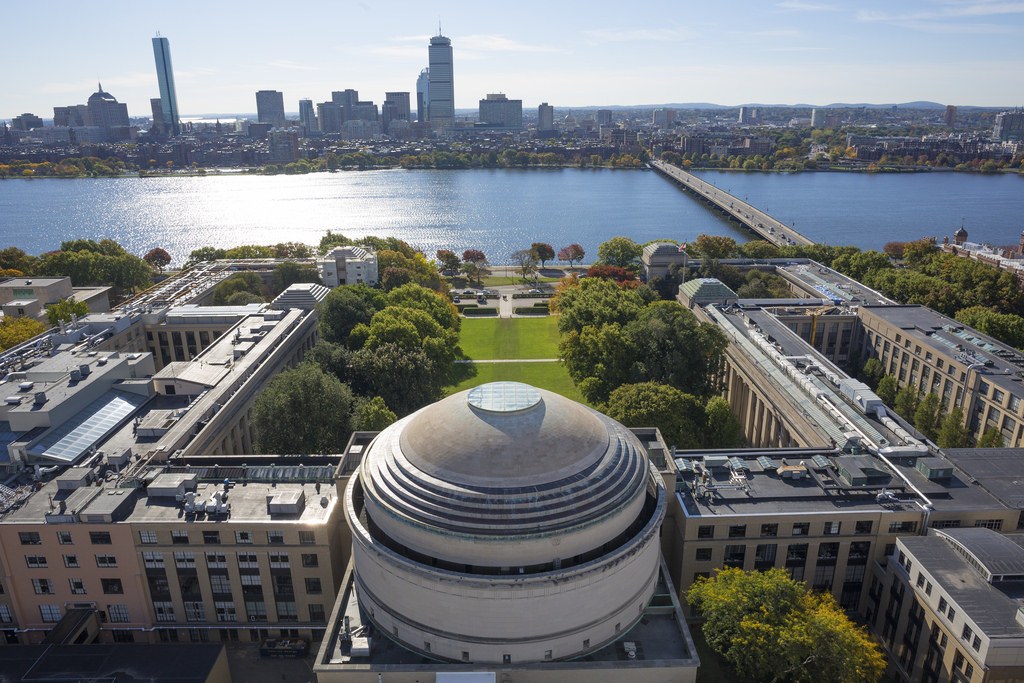
\includegraphics[width=0.9\textwidth]{anh/MIT.jpg}
            \caption{Viện Công nghệ Massachusetts (MIT)}
        \end{figure}
    \end{minipage}\hfill
    \begin{minipage}{0.5\textwidth}
        \begin{figure}
            \centering
            
\includegraphics[width=0.9\textwidth]{anh/CMU.jpg}
            \caption{Đại học Carnegie Mellon}
        \end{figure}
    \end{minipage}
\end{frame}
\end{document}